\documentclass{beamer}
% \usepackage[utf8]{inputenc}

\usepackage{amsmath, amsfonts, amssymb}
\usepackage{amsthm}
\usepackage{mathtools}
\usepackage{physics}
\usepackage[super]{nth}

\usepackage{graphicx}
\graphicspath{{../assets/}}

\usepackage{pgfplots}
\usepackage{tikz}
\usepackage{standalone}

\newcommand{\ee}{\operatorname{e}}          % Euler's number
\newcommand{\ii}{\mathrm{i}}                % imaginary unit
\newcommand{\ad}[1]{a_{#1}^{\dagger}}       % creation operator
\newcommand*\mean[1]{\overline{#1}}         % mean

\usetheme{metropolis}           % Use metropolis theme
\usepackage{appendixnumberbeamer}
\title{Large-Scale Numerical Investigations into the Dynamics of Nonlinear Classical Systems}
\date{\today}
\author{Sebastian Micluța-Câmpeanu}
\institute{University of Bucharest}
\begin{document}
\maketitle

%%%%%%%%%%%%%%%%%%%%%%%%%%%% slide 1 %%%%%%%%%%%%%%%%%%%%%%%%%%%%

\begin{frame}{Outline}
  \tableofcontents[]
\end{frame}

%%%%%%%%%%%%%%%%%%%%%%%%%%%% slide 2 %%%%%%%%%%%%%%%%%%%%%%%%%%%%

\begin{frame}{Acknowledgements}
	\begin{itemize}
		\item I would like to thank A.I.~Nicolin, and V.~Băran for helping and motivating me.
		\item The author has been	supported by PN-III-P4-ID-PCE-2016-0792.
		\item All numerical simulations were performed on the computing cluster of
		Department of Computational Physics and Information Technologies,
		``Horia Hulubei'' National Institute for Physics and Nuclear Engineering.
	\end{itemize}
\end{frame}

\section{Introduction}

%%%%%%%%%%%%%%%%%%%%%%%%%%%% slide 3 %%%%%%%%%%%%%%%%%%%%%%%%%%%%

\begin{frame}{The model}
  \begin{itemize}
		\item The physical system that we model is the surface of heavy nuclei.
    \item The Hamiltonian describes the constrained motion of the vibrational quadrupole degrees of freedom of nuclear surface.
  \end{itemize}
\end{frame}

%%%%%%%%%%%%%%%%%%%%%%%%%%%% slide 4 %%%%%%%%%%%%%%%%%%%%%%%%%%%%

\begin{frame}{The model}
	The Hamiltonian of the system
	\begin{equation*}
    H = \alert<1,2>{\frac{A}{2}\left(p_0^2+p_2^2\right)+\frac{A}{2}\left(q_0^2+q_2^2\right)}
		 +\alert<3>{\frac{B}{\sqrt{2}}q_0\left(3q_2^2-q_0^2\right)}
		 +\alert<2>{\frac{D}{4}\left(q_0^2+q_2^2\right)^2}
  \end{equation*}

	\begin{columns}
		\column{0.5\textwidth}
		\begin{itemize}
			\item \alert<1> {Harmonic oscillator part}
			\item \alert<2> {Integrable part}
			\item \alert<3> {Non-integrable term}
		\end{itemize}

		\column{0.5\textwidth}
		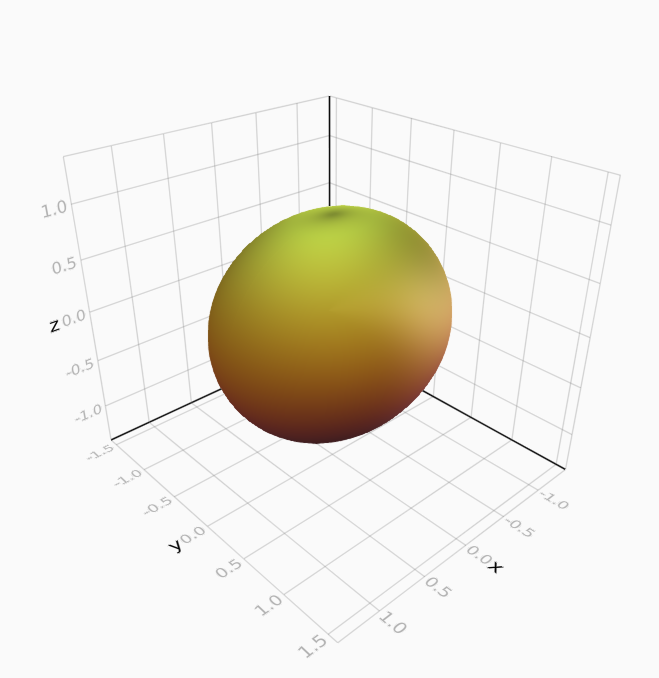
\includegraphics[width=\textwidth]{nucleus}
	\end{columns}
\end{frame}

%%%%%%%%%%%%%%%%%%%%%%%%%%%% slide 5 %%%%%%%%%%%%%%%%%%%%%%%%%%%%


\begin{frame}
	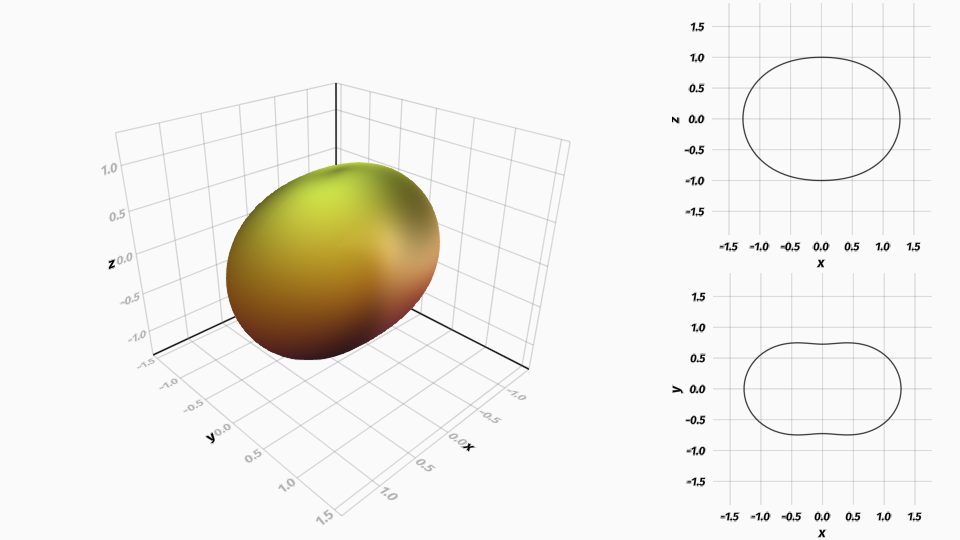
\includegraphics[width=\textwidth]{nucleus-with-sections}
\end{frame}

%%%%%%%%%%%%%%%%%%%%%%%%%%%% slide 6 %%%%%%%%%%%%%%%%%%%%%%%%%%%%

\begin{frame}
	\begin{figure}
		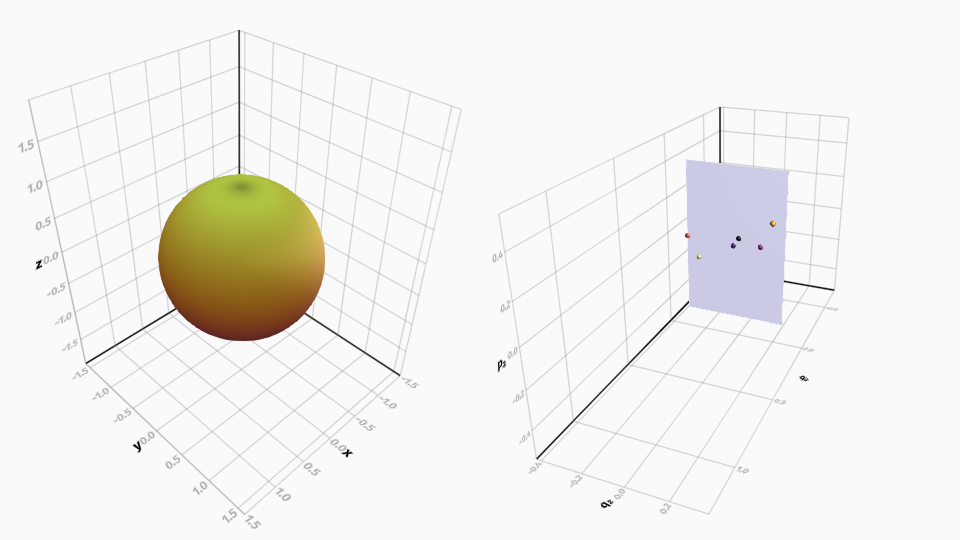
\includegraphics[width=\textwidth]{nucleus-with-poincare}
		\caption{The nucleus and the Poincaré section at \(B=0.5, E=0.3\)}
	\end{figure}
\end{frame}

\section{Numerical simulations}

%%%%%%%%%%%%%%%%%%%%%%%%%%%% slide 7 %%%%%%%%%%%%%%%%%%%%%%%%%%%%

\begin{frame}
	\begin{figure}
		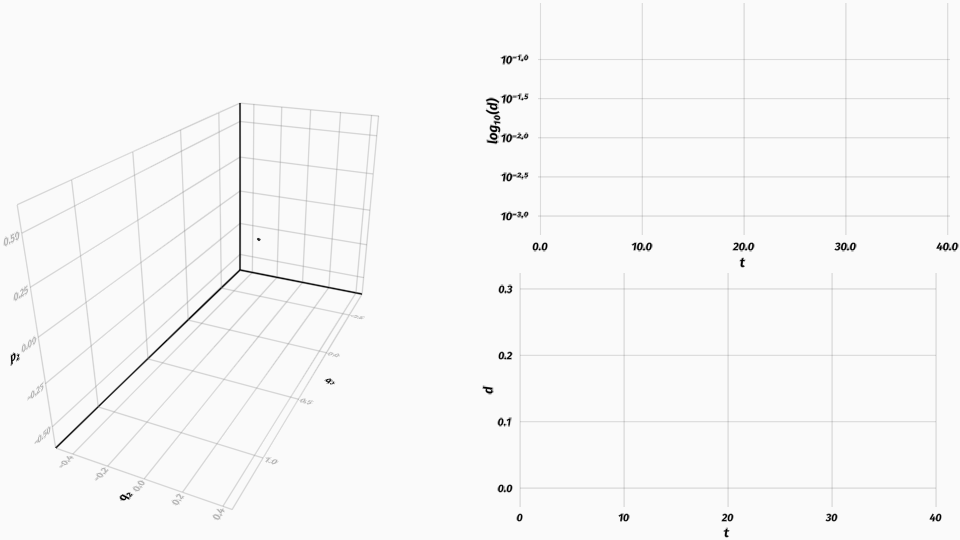
\includegraphics[width=\textwidth]{dist-with-log}
		\caption{The distance between nearby trajectories for \(B=0.5, E=0.3\)}
	\end{figure}
\end{frame}

%%%%%%%%%%%%%%%%%%%%%%%%%%%% slide 8 %%%%%%%%%%%%%%%%%%%%%%%%%%%%

\begin{frame}
	\begin{figure}
		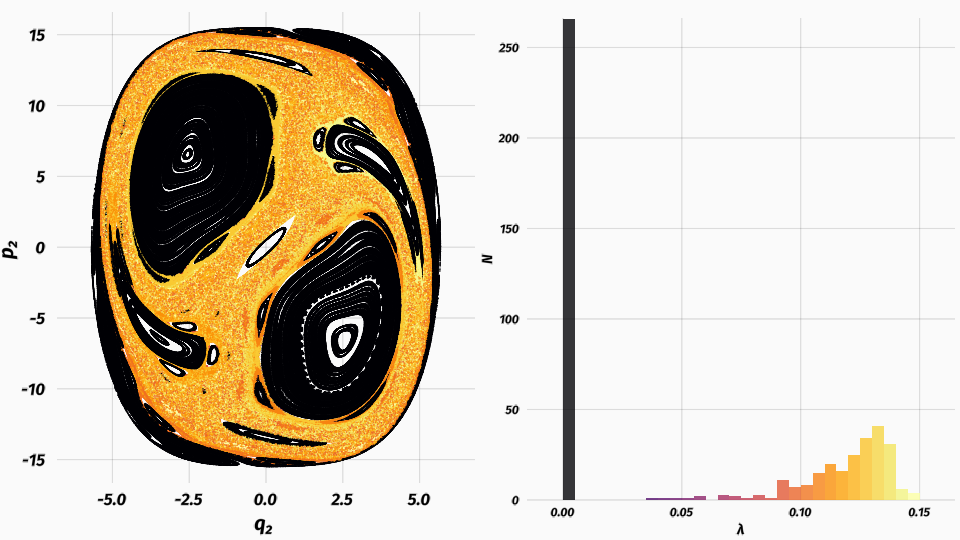
\includegraphics[width=\textwidth]{poincare}
		\caption{A Poincaré section at \(B=0.55, E=120\)}
	\end{figure}
\end{frame}

%%%%%%%%%%%%%%%%%%%%%%%%%%%% slide 9 %%%%%%%%%%%%%%%%%%%%%%%%%%%%

\begin{frame}
	\begin{figure}
		\includestandalone[width=\textwidth]{../assets/short-benchmark-E}
		\caption{Energy error benchmark for short integration time}
	\end{figure}
\end{frame}

%%%%%%%%%%%%%%%%%%%%%%%%%%%% slide 10 %%%%%%%%%%%%%%%%%%%%%%%%%%%%

\begin{frame}
	\begin{figure}
		\includestandalone[width=\textwidth]{../assets/short-benchmark-t}
		\caption{Computational time benchmark for short integration time}
	\end{figure}
\end{frame}

%%%%%%%%%%%%%%%%%%%%%%%%%%%% slide 11 %%%%%%%%%%%%%%%%%%%%%%%%%%%%

\begin{frame}
	\begin{figure}
		\includestandalone[width=\textwidth]{../assets/long-benchmark-E}
		\caption{Energy error benchmark for long integration time}
	\end{figure}
\end{frame}

%%%%%%%%%%%%%%%%%%%%%%%%%%%% slide 12 %%%%%%%%%%%%%%%%%%%%%%%%%%%%

\begin{frame}
	\begin{figure}
		\includestandalone[width=\textwidth]{../assets/long-benchmark-t}
		\caption{Computational time benchmark for long integration time}
	\end{figure}
\end{frame}

%%%%%%%%%%%%%%%%%%%%%%%%%%%% slide 13 %%%%%%%%%%%%%%%%%%%%%%%%%%%%

\begin{frame}
	\begin{figure}
		\includestandalone[width=\textwidth]{../assets/hist-lambda-4}
		\caption{Maximal Lyapunov coefficient histogram for \(B=0.5, E=120\).}
	\end{figure}
\end{frame}

%%%%%%%%%%%%%%%%%%%%%%%%%%%% slide 14 %%%%%%%%%%%%%%%%%%%%%%%%%%%%

\begin{frame}
	\begin{figure}
		\includestandalone[width=\textwidth]{../assets/hist-lambda-5}
		\caption{Maximal Lyapunov coefficient histogram for \(B=0.5, E=120\).}
	\end{figure}
\end{frame}

%%%%%%%%%%%%%%%%%%%%%%%%%%%% slide 15 %%%%%%%%%%%%%%%%%%%%%%%%%%%%

\begin{frame}
	\begin{figure}
		\includestandalone[width=\textwidth]{../assets/hist-lambda-6}
		\caption{Maximal Lyapunov coefficient histogram for \(B=0.5, E=120\).}
	\end{figure}
\end{frame}

%%%%%%%%%%%%%%%%%%%%%%%%%%%% slide 16 %%%%%%%%%%%%%%%%%%%%%%%%%%%%

\begin{frame}
	\begin{figure}
		\includestandalone[width=\textwidth]{../assets/hist-lambda-7}
		\caption{Maximal Lyapunov coefficient histogram for \(B=0.5, E=120\).}
	\end{figure}
\end{frame}

%%%%%%%%%%%%%%%%%%%%%%%%%%%% slide 17 %%%%%%%%%%%%%%%%%%%%%%%%%%%%

\begin{frame}
	\begin{figure}
		\includestandalone[width=\textwidth]{../assets/hist-lambda-selected-before}
		\caption{Selecting the chaotic trajectories for \(B=0.5, E=120\).}
	\end{figure}
\end{frame}

%%%%%%%%%%%%%%%%%%%%%%%%%%%% slide 18 %%%%%%%%%%%%%%%%%%%%%%%%%%%%

\begin{frame}
	\begin{figure}
		\includestandalone[width=\textwidth]{../assets/hist-lambda-selected-after}
		\caption{Selecting the chaotic trajectories for \(B=0.5, E=120\).}
	\end{figure}
\end{frame}

%%%%%%%%%%%%%%%%%%%%%%%%%%%% slide 19 %%%%%%%%%%%%%%%%%%%%%%%%%%%%

\begin{frame}
	\begin{figure}
		\includestandalone[width=\textwidth]{../assets/mean-over-ic}
		\caption{Averaged \(\lambda\) for \(B=0.5, E \in (10, 3000)\).}
	\end{figure}
\end{frame}

%%%%%%%%%%%%%%%%%%%%%%%%%%%% slide 20 %%%%%%%%%%%%%%%%%%%%%%%%%%%%

\begin{frame}
	\begin{figure}
		\includestandalone[width=\textwidth]{../assets/mean-over-ic-low}
		\caption{Averaged \(\lambda\) for \(B=0.5, E \in (0.01, 10)\).}
	\end{figure}
\end{frame}

%%%%%%%%%%%%%%%%%%%%%%%%%%%% slide 21 %%%%%%%%%%%%%%%%%%%%%%%%%%%%

\begin{frame}
	\begin{figure}
		\includestandalone[width=\textwidth]{../assets/mean-over-E}
		\caption{Averaged \(\lambda\) for \(B=0.5, E \in (10, 3000)\)
		and \(B \in (0.1, 0.6)\).}
	\end{figure}
\end{frame}

%%%%%%%%%%%%%%%%%%%%%%%%%%%% slide 22 %%%%%%%%%%%%%%%%%%%%%%%%%%%%

\begin{frame}
	\begin{figure}
		\includestandalone[width=\textwidth]{../assets/mean-over-E-low}
		\caption{Averaged \(\lambda\) for \(B=0.5, E \in (0.01, 10)\)
		and \(B \in (0.1, 0.6)\).}
	\end{figure}
\end{frame}

%%%%%%%%%%%%%%%%%%%%%%%%%%%% slide 23 %%%%%%%%%%%%%%%%%%%%%%%%%%%%

\begin{frame}
	\begin{figure}
		\includestandalone[width=\textwidth]{../assets/mean-over-ic-dinf}
		\caption{Averaged \(d_\infty\) for \(B=0.5, E \in (10, 3000)\).}
	\end{figure}
\end{frame}

%%%%%%%%%%%%%%%%%%%%%%%%%%%% slide 24 %%%%%%%%%%%%%%%%%%%%%%%%%%%%

\begin{frame}
	\begin{figure}
		\includestandalone[width=\textwidth]{../assets/mean-over-ic-low-dinf}
		\caption{Averaged \(d_\infty\) for \(B=0.5, E \in (0.01, 10)\).}
	\end{figure}
\end{frame}

%%%%%%%%%%%%%%%%%%%%%%%%%%%% slide 24 %%%%%%%%%%%%%%%%%%%%%%%%%%%%

\begin{frame}
	\begin{figure}
		\includestandalone[width=\textwidth]{../assets/mean-over-ic-Gamma}
		\caption{Averaged \(\Gamma\) for \(B=0.5, E \in (10, 3000)\).}
	\end{figure}
\end{frame}

%%%%%%%%%%%%%%%%%%%%%%%%%%%% slide 25 %%%%%%%%%%%%%%%%%%%%%%%%%%%%

\begin{frame}
	\begin{figure}
		\includestandalone[width=\textwidth]{../assets/mean-over-ic-low-Gamma}
		\caption{Averaged \(\Gamma\) for \(B=0.5, E \in (0.01, 10)\).}
	\end{figure}
\end{frame}

%%%%%%%%%%%%%%%%%%%%%%%%%%%% slide 26 %%%%%%%%%%%%%%%%%%%%%%%%%%%%

\section{Conclusions}

\begin{frame}[standout]
Thank you!
\end{frame}

\appendix

%%%%%%%%%%%%%%%%%%%%%%%%%%%% slide a1 %%%%%%%%%%%%%%%%%%%%%%%%%%%%

\begin{frame}
	\begin{figure}
		\includestandalone[width=\textwidth]{../assets/short-benchmark-rescaling-E}
		\caption{Energy error benchmark for short integration time with rescaling}
	\end{figure}
\end{frame}

%%%%%%%%%%%%%%%%%%%%%%%%%%%% slide a2 %%%%%%%%%%%%%%%%%%%%%%%%%%%%

\begin{frame}
	\begin{figure}
		\includestandalone[width=\textwidth]{../assets/short-benchmark-rescaling-t}
		\caption{Computational time benchmark for short integration time with rescaling}
	\end{figure}
\end{frame}

%%%%%%%%%%%%%%%%%%%%%%%%%%%% slide a3 %%%%%%%%%%%%%%%%%%%%%%%%%%%%

\begin{frame}
	\begin{figure}
		\includestandalone[width=\textwidth]{../assets/long-benchmark-rescaling-E}
		\caption{Energy error benchmark for long integration time with rescaling}
	\end{figure}
\end{frame}

%%%%%%%%%%%%%%%%%%%%%%%%%%%% slide a4 %%%%%%%%%%%%%%%%%%%%%%%%%%%%

\begin{frame}
	\begin{figure}
		\includestandalone[width=\textwidth]{../assets/long-benchmark-rescaling-t}
		\caption{Computational time benchmark for long integration time with rescaling}
	\end{figure}
\end{frame}

%%%%%%%%%%%%%%%%%%%%%%%%%%%% slide a5 %%%%%%%%%%%%%%%%%%%%%%%%%%%%

\begin{frame}[fragile]{Backup slides}
  Sometimes, it is useful to add slides at the end of your presentation to
  refer to during audience questions.


\end{frame}

\begin{frame}[allowframebreaks]{References}

  \bibliography{demo}
  \bibliographystyle{abbrv}

\end{frame}

\end{document}
